% THIS DOCUMENT IS FOLLOWS THE VOLERE TEMPLATE BY Suzanne Robertson and James Robertson
% ONLY THE SECTION HEADINGS ARE PROVIDED
%
% Initial draft from https://github.com/Dieblich/volere
%
% Risks are removed because they are covered by the Hazard Analysis
\documentclass[12pt]{article}

\usepackage{booktabs}
\usepackage{tabularx}
\usepackage{hyperref}
\usepackage{graphicx}

\hypersetup{
    bookmarks=true,         % show bookmarks bar?
      colorlinks=true,      % false: boxed links; true: colored links
    linkcolor=red,          % color of internal links (change box color with linkbordercolor)
    citecolor=green,        % color of links to bibliography
    filecolor=magenta,      % color of file links
    urlcolor=cyan           % color of external links
}

\newcommand{\lips}{\textit{Insert your content here.}}

%% Comments

\usepackage{color}

\newif\ifcomments\commentstrue %displays comments
%\newif\ifcomments\commentsfalse %so that comments do not display

\ifcomments
\newcommand{\authornote}[3]{\textcolor{#1}{[#3 ---#2]}}
\newcommand{\todo}[1]{\textcolor{red}{[TODO: #1]}}
\else
\newcommand{\authornote}[3]{}
\newcommand{\todo}[1]{}
\fi

\newcommand{\wss}[1]{\authornote{blue}{SS}{#1}} 
\newcommand{\plt}[1]{\authornote{magenta}{TPLT}{#1}} %For explanation of the template
\newcommand{\an}[1]{\authornote{cyan}{Author}{#1}}

%% Common Parts

\newcommand{\progname}{Software Engineering} % PUT YOUR PROGRAM NAME HERE
\newcommand{\authname}{Team 8 -- Rhythm Rangers\\
\\ Ansel Chen
\\ Muhammad Jawad
\\ Mohamad-Hassan Bahsoun
\\ Matthew Baleanu
\\ Ahmed Al-Hayali} % AUTHOR NAMES                  

\usepackage{hyperref}
    \hypersetup{colorlinks=true, linkcolor=blue, citecolor=blue, filecolor=blue,
                urlcolor=blue, unicode=false}
    \urlstyle{same}
                                


\begin{document}

\title{Software Requirements Specification for \progname: subtitle describing software} 
\author{\authname}
\date{\today}
	
\maketitle

~\newpage

\pagenumbering{roman}

\tableofcontents

~\newpage

\section*{Revision History}

\begin{tabularx}{\textwidth}{p{3cm}p{2cm}X}
\toprule {\textbf{Date}} & {\textbf{Version}} & {\textbf{Notes}}\\
\midrule
Date 1 & 1.0 & Notes\\
Date 2 & 1.1 & Notes\\
\bottomrule
\end{tabularx}

~\\

~\newpage
\section{Purpose of the Project}
\subsection{User Business}
\lips
\subsection{Goals of the Project}
\lips
\section{Stakeholders}
\subsection{Client}
\lips
\subsection{Customer}
\lips
\subsection{Other Stakeholders}
\lips
\subsection{Hands-On Users of the Project}
\lips
\subsection{Personas}
\lips
\subsection{Priorities Assigned to Users}
\lips
\subsection{User Participation}
\lips
\subsection{Maintenance Users and Service Technicians}
\lips

\section{Mandated Constraints}
\subsection{Solution Constraints}
\begin{itemize}
  \item Constraint
  \\ \textbf{Rationale:} 
  \\ \textbf{Fit Criterion:} 

  \item The Service shall handle user interaction through a web application.
  \\\textbf{Rationale}: allows for users to access the service through any device with an internet connection
  \\\textbf{Fit Criterion}: the web application functions correctly on both a mobile phone browser and PC. 

  \item The service uses a music dataset, such as openAI's jukebox dataset. 
  \\ \textbf{Rationale:} A dataset for an AI project is necessary as some form of training data must be used 
  in order to train the AI generative, analysis and recommendation systems. 
  \\ \textbf{Fit Criterion:} The system uses a music dataset as the training source. 

  \item The service uses a cloud infrastructure for computations.
  \\ \textbf{Rationale:} The cloud infrastructure is scalable and allows for computation for the AI portions
  of the project to not be done locally. 
  \\ \textbf{Fit Criterion:} The system must be deployed on a form of a cloud platform (such as AWS), and utilize the platform for some features
  such as the machine learning components. 

  \item The service uses a modern database system. 
  \\ \textbf{Rationale:} A database system would allow the service to store user data, song metadata, it can act like a pseudo-cache for performance. 
  \\ \textbf{Fit Criterion:} A database that stores music metadata must be deployed. 
  

\end{itemize}

\subsection{Implementation Environment of the Current System}
\begin{itemize}
  \item Cloud Hosting Infrastructure
  \\ \textbf{Rationale:} Cloud hosting can allow the service to remotely store user and service information, in addition to AI machine learning 
  features.

  \item Computational Resources Available for the Service/Hardware Constraints
  \\ \textbf{Rationale:} The computational resources accessible for both the training and service provision to the user must be considered. 
  This can include, but is not limited to how powerful the CPU, GPU that can be used to train the machine learning model and what level of
  computational power the end user has on hand determines how much resources the services can use to give the user their desired results. 

  \item Storage/Database Systems
  \\ \textbf{Rationale:} How the training data and user data is trained are both very important considerations. This can include both using some form
  of a cloud storage or local database. 

  \item Network Constraints
  \\ \textbf{Rationale:} The system will likely require a fast, high-bandwidth internet connections because the user is expected to upload music or references 
  to said music before the service responds to the user request. This means an efficient method of allowing users to upload said references is 
  important, as the user uploading entire music files might greatly reduce the amount of music that can be fed into the final service (as some
  of said music files would likely be illegally obtained) and would require uploading far too much data, thus slowing the entire process down.

  \item External Resources Constraints
  \\ \textbf{Rationale:} The service will most likely have to access an external API, such as spotify's, which already includes a lot of 
  useful information that can be provided for the service in order to function. Whether these are available or not, or how expensive the API
  calls actually are can greatly affect the viability of certain aspects of the project. This also includes open source music data sets for
  a machine learning project, it is possible those sets only contain a certain type of music (such as electronic) and does not feature a lot of
  hip hop, which can prevent the service from effectively engaging with certain types of sound or genre. 

  \item Security Constraints
  \\ \textbf{Rationale:} Security protocols to protect a potential remote server the service employs and preventing unauthorized access to 
  user data are both potentially very important elements of the service that need to be considered. 

  \item Liscensing Constraints 
  \\ \textbf{Rationale:} Currently, there is an ongoing debate over whether AI generation, especially related to art, can be considered 
  as plagiarism or intellectual properthy theft. If the machine learning components of the service is trained on music from a large artist 
  that does not approve of the end project, it is possible that there would be some form of legal consequences, thus the selection of 
  trianing data and what songs the user is allowed to input into the final model needs to be seriously considered. 

\end{itemize}

\subsection{Partner or Collaborative Applications}

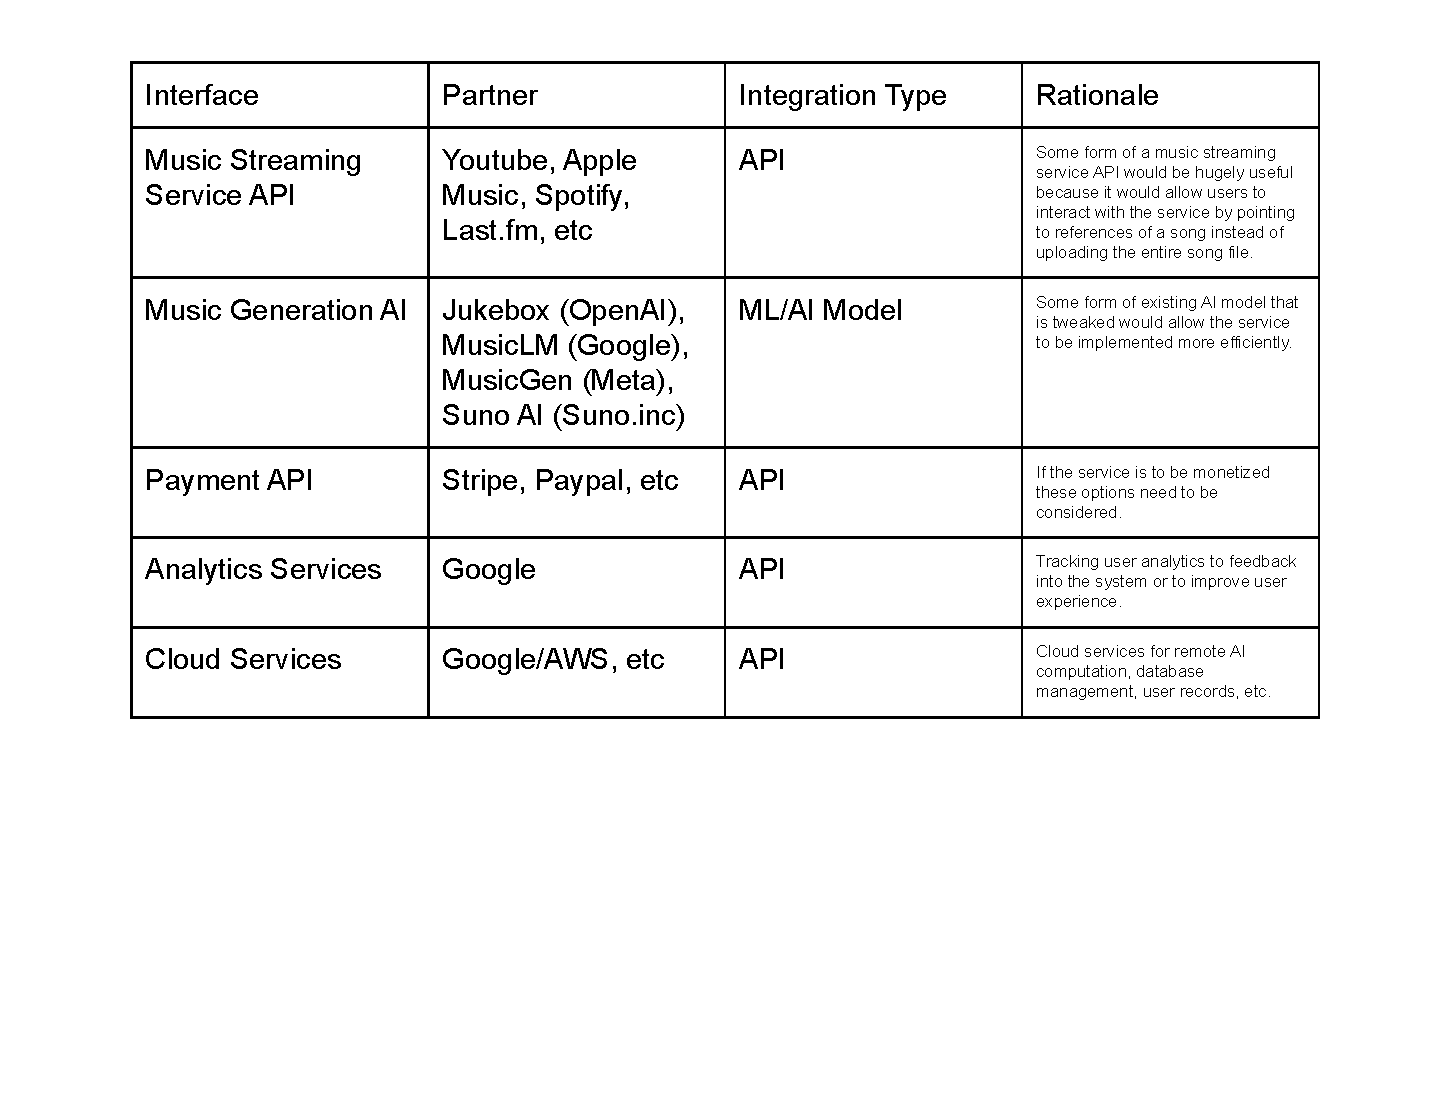
\includegraphics[scale=0.72]{3_3_partner_constraints_figure}


\subsection{Off-the-Shelf Software}
\begin{itemize}
  \item Constraint
  \\ \textbf{Rationale:} 
  \\ \textbf{Fit Criterion:} 
\end{itemize}

\subsection{Anticipated Workplace Environment}
\begin{itemize}
  \item Constraint
  \\ \textbf{Rationale:} 
  \\ \textbf{Fit Criterion:} 
\end{itemize}

\subsection{Schedule Constraints}
\begin{itemize}
  \item Constraint
  \\ \textbf{Rationale:} 
  \\ \textbf{Fit Criterion:} 
\end{itemize}

\subsection{Budget Constraints}
\begin{itemize}
  \item Constraint
  \\ \textbf{Rationale:} 
  \\ \textbf{Fit Criterion:} 
\end{itemize}

\subsection{Enterprise Constraints}
\begin{itemize}
  \item Constraint
  \\ \textbf{Rationale:} 
  \\ \textbf{Fit Criterion:} 
\end{itemize}

\section{Naming Conventions and Terminology}
\subsection{Glossary of All Terms, Including Acronyms, Used by Stakeholders
involved in the Project}
\lips

\section{Relevant Facts And Assumptions}
\subsection{Relevant Facts}
\lips
\subsection{Business Rules}
\lips
\subsection{Assumptions}
\lips

\section{The Scope of the Work}
\subsection{The Current Situation}
\lips
\subsection{The Context of the Work}
\lips
\subsection{Work Partitioning}
\lips
\subsection{Specifying a Business Use Case (BUC)}
\lips

\section{Business Data Model and Data Dictionary}
\subsection{Business Data Model}
\lips
\subsection{Data Dictionary}
\lips

\section{The Scope of the Product}
\subsection{Product Boundary}
\lips
\subsection{Product Use Case Table}
\lips
\subsection{Individual Product Use Cases (PUC's)}
\lips

\section{Functional Requirements}
\subsection{Functional Requirements}
\lips

\section{Look and Feel Requirements}
\subsection{Appearance Requirements}
\lips
\subsection{Style Requirements}
\lips

\section{Usability and Humanity Requirements}
\subsection{Ease of Use Requirements}
\lips
\subsection{Personalization and Internationalization Requirements}
\lips
\subsection{Learning Requirements}
\lips
\subsection{Understandability and Politeness Requirements}
\lips
\subsection{Accessibility Requirements}
\lips

\section{Performance Requirements}
\subsection{Speed and Latency Requirements}
\lips
\subsection{Safety-Critical Requirements}
\lips
\subsection{Precision or Accuracy Requirements}
\lips
\subsection{Robustness or Fault-Tolerance Requirements}
\lips
\subsection{Capacity Requirements}
\lips
\subsection{Scalability or Extensibility Requirements}
\lips
\subsection{Longevity Requirements}
\lips

\section{Operational and Environmental Requirements}
\subsection{Expected Physical Environment}
\lips
\subsection{Wider Environment Requirements}
\lips
\subsection{Requirements for Interfacing with Adjacent Systems}
\lips
\subsection{Productization Requirements}
\lips
\subsection{Release Requirements}
\lips

\section{Maintainability and Support Requirements}
\subsection{Maintenance Requirements}
\lips
\subsection{Supportability Requirements}
\lips
\subsection{Adaptability Requirements}
\lips

\section{Security Requirements}
\subsection{Access Requirements}
\lips
\subsection{Integrity Requirements}
\lips
\subsection{Privacy Requirements}
\lips
\subsection{Audit Requirements}
\lips
\subsection{Immunity Requirements}
\lips

\section{Cultural Requirements}
\subsection{Cultural Requirements}
\lips

\section{Compliance Requirements}
\subsection{Legal Requirements}
\lips
\subsection{Standards Compliance Requirements}
\lips

\section{Open Issues}
\lips

\section{Off-the-Shelf Solutions}
\subsection{Ready-Made Products}
\lips
\subsection{Reusable Components}
\lips
\subsection{Products That Can Be Copied}
\lips

\section{New Problems}
\subsection{Effects on the Current Environment}
\lips
\subsection{Effects on the Installed Systems}
\lips
\subsection{Potential User Problems}
\lips
\subsection{Limitations in the Anticipated Implementation Environment That May
Inhibit the New Product}
\lips
\subsection{Follow-Up Problems}
\lips

\section{Tasks}
\subsection{Project Planning}
\lips
\subsection{Planning of the Development Phases}
\lips

\section{Migration to the New Product}
\subsection{Requirements for Migration to the New Product}
\lips
\subsection{Data That Has to be Modified or Translated for the New System}
\lips

\section{Costs}
\lips
\section{User Documentation and Training}
\subsection{User Documentation Requirements}
\lips
\subsection{Training Requirements}
\lips

\section{Waiting Room}
\lips

\section{Ideas for Solution}
\lips

\newpage{}
\section*{Appendix --- Reflection}

The information in this section will be used to evaluate the team members on the
graduate attribute of Lifelong Learning.  Please answer the following questions:

\begin{enumerate}
  \item What knowledge and skills will the team collectively need to acquire to
  successfully complete this capstone project?  Examples of possible knowledge
  to acquire include domain specific knowledge from the domain of your
  application, or software engineering knowledge, mechatronics knowledge or
  computer science knowledge.  Skills may be related to technology, or writing,
  or presentation, or team management, etc.  You should look to identify at
  least one item for each team member.
  \item For each of the knowledge areas and skills identified in the previous
  question, what are at least two approaches to acquiring the knowledge or
  mastering the skill?  Of the identified approaches, which will each team
  member pursue, and why did they make this choice?
\end{enumerate}

\end{document}